In statistics, principal component analysis (PCA) is a technique used to describe a data set in terms of new, uncorrelated variables (components). Components are ordered by the amount of original variance they describe, so the technique is useful for reducing the dimensionality of a data set. Each of them is a linear combination of the set of features of the system. Therefore, if we know the weight assigned to each characteristic of the system, we are able to deduce the ``importance'' of each feature weighted by an specific explained variance.

For the PCA, the normalized data will not be enough. Of course, it will be necessary to replace the missing values as we explained in Section \ref{sect:DatPrep}, but also we are going to require a set of data with its features centred in zero, that is to say, that their mean must be zero. This transformation is called standardisation and we will apply it to our dataset.

If the PCA is executed with as many components as features, the sum of the explained cumulative variance ratio of all components is always 1. In other words, if all the main components of a dataset are calculated, then, although transformed, all the information present in the original data is being stored. With this method, we are able to know the various components that we can obtain and their explained variance. Likewise, the behaviour of the cumulative variance ratio is defined by the curve shown in Figure \ref{fig:cumexpvar}.

\begin{figure}
	\centering%
	\centerline{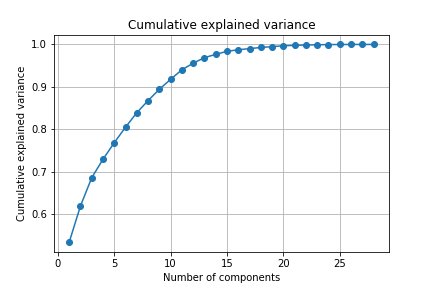
\includegraphics[width=0.7\textwidth]{Imagenes/Bitmap/PCA/cumexpvar.png}}%
	\caption{Evolution of cumulative explained variance ratio}%
	\label{fig:cumexpvar}
\end{figure}

Looking at Figure \ref{fig:cumexpvar}, we can affirm that around the 10 components, the increase of the explained accumulated variance stops being substantial and we reach a reasonable value of it. Hence, with the observed curve we are able to determine the suitable number of components. However, before delving into each of the components, let's study in more detail the distribution of the variance explained. For this purpose, we are going to represent the distribution of explained variance in a pie chart with which it will be easier for us to compare the different values of it. This graph is shown in Figure \ref{fig:expvarpie}.

\begin{figure}
	\centering%
	\centerline{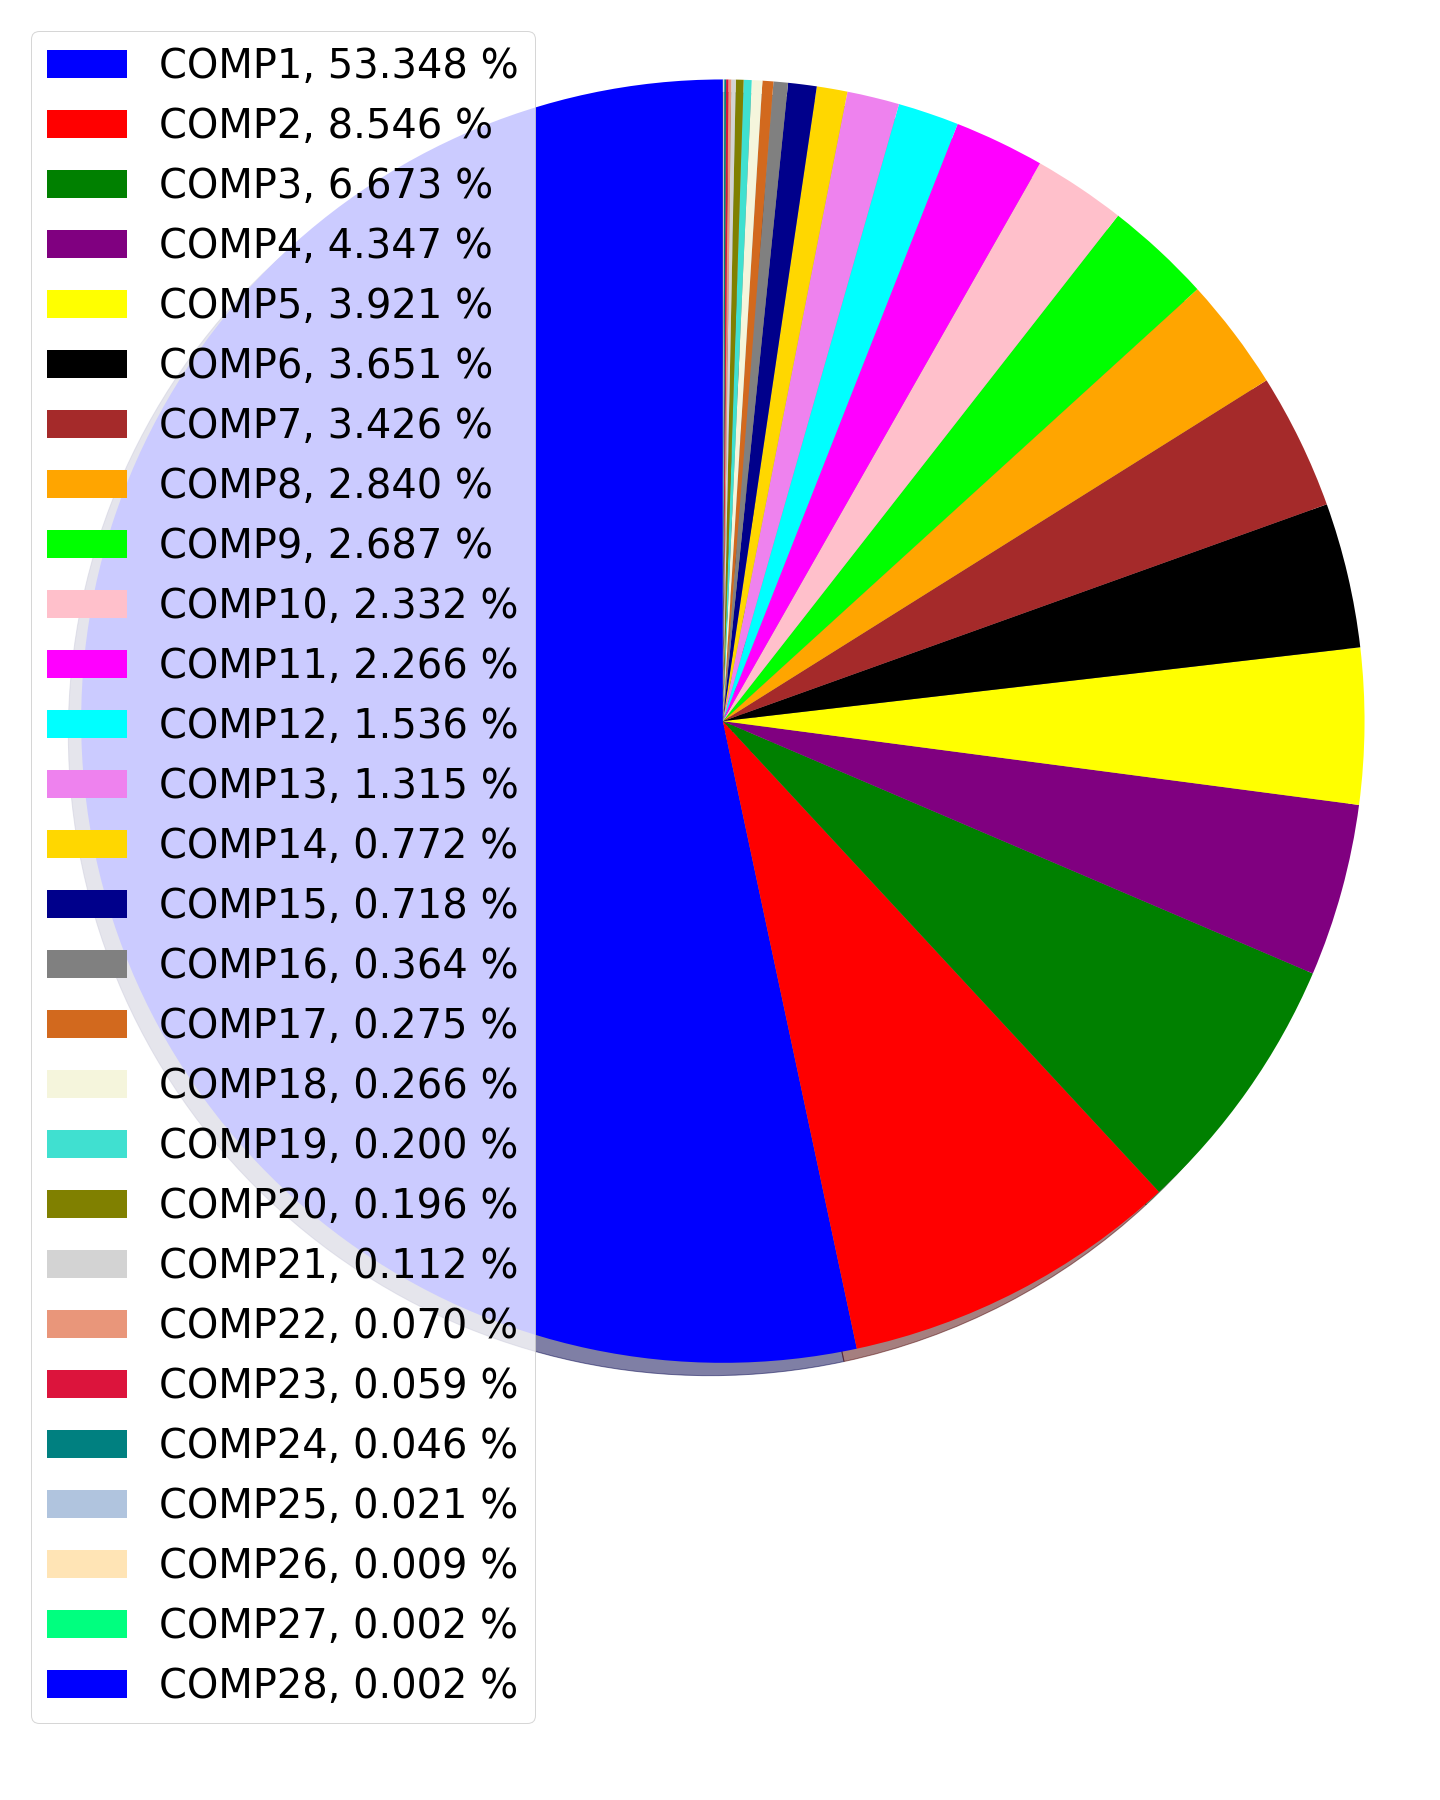
\includegraphics[width=0.5\textwidth]{Imagenes/Bitmap/PCA/expvarpie.png}}%
	\caption{Distribution of explained variance ratio}%
	\label{fig:expvarpie}
\end{figure}

Taking advantage of the information provided by the last graphic (Figure \ref{fig:expvarpie}) we can observe that the only component that has an explained variance ratio bigger than $10$\% is the first one. Besides, from the fourth one all of them has a value smaller than 5\% and from the thirteenth one the components have a poorly significant value. Nevertheless, we have to take into account that, given the distribution of our classification (see Figure \ref{fig:distr}), the losing of a small percentage of explained variance may mean missing information related to categories with few elements. This results from the fact that the PCA does not consider the appropriate classification during its execution.

In spite of the explained results in terms of components distribution, we could expect to obtain more clarifying values in the weights that define the components with higher explained variance ratio. Therefore, we will now know the linear combination of the first component with respect to the characteristics explained.

The best way to visualise the different linear combination weights is through a pie chart. This is because, with this graph, it is easy to compare the importance given to each dimension. In our Figure \ref{fig:comp0pie}, we have striped each linear combination which has a a negative weight and represented the absolute values of all coefficient. Since we are not so interested in the sense of each dimension in the definition of the first component, we will calculate the direction ratio that is assigned to each characteristic, for example if our system had two features (which is the same as saying that the system has two dimensions) and the direction ratio was greater in the first one, which we can represent on the abscissa axis, we would obtain a vectorial component whose representation in the common Cartesian plane will be ``more horizontal than vertical'', since the weight assigned to that dimension is greater. To find this direction ratio, we will divide the absolute value of the coefficient by the sum of the absolute value of each of the weights, that is to say, if a component is defined as follows:

$$
c_{i, k} = \sum_{j = 0}^N\lambda_{i, j}x_{k, j}
$$

Where $c_{i, k}$ is the value of the i-th component of the k-th e-mail, $N$ is the number of dimensions (28 in our case), $\lambda_{i, j}\in\mathds{R}$ is the linear combination coefficient (also called weight) of the i-th component for the j-th dimension and $x_{k, j}$ represents the j-th feature of the k-th message. Then, the direction ratio of the j-th characteristic of the i-th component is as follows:

$$
d_j = \frac{\lvert\lambda_{i,j}\rvert}{\sum_{j = 0}^N\lvert\lambda_{i, j}\rvert}
$$

The result of this operation will be the percentages that we can find next to each characteristic in the Figure \ref{fig:comp0pie}.

\begin{figure}
	\centering%
	\centerline{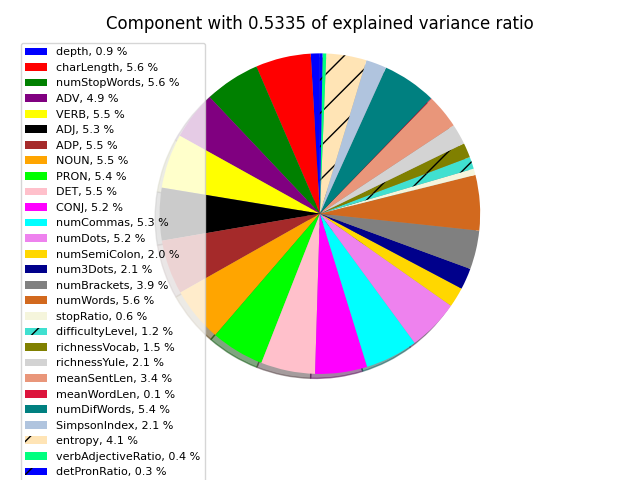
\includegraphics[width=0.9\textwidth]{Imagenes/Bitmap/PCA/comp0pie.png}}%
	\caption{Linear combination that defines the first component}%
	\label{fig:comp0pie}
\end{figure}

In addition to the problems of the choice about the number of components given our distribution in categories, we have a balanced assignment of weights of almost all the features in the first component, which has the highest explained variance with a ratio of 53.35\%. These information does not allow us to determine which style markers differentiate the categories of the messages. Furthermore, by not taking into account our classification, we can only state that the assignment of coefficients of the linear combination that defines the first component distinguishes the elements of the set equally, regardless of the class to which they belong.

As the rest of the components have an explained variance ratio smaller that 0.1, their direction ratios will not be sufficiently representative to overcome such a balanced distribution. For this reason, we can conclude that it is necessary to look for other method of dimension reduction which provides us information taking into account our classification and allows us to know which style metrics describe the different categories in the best possible way.